\documentclass{article}[18pt]
\ProvidesPackage{format}
%Page setup
\usepackage[utf8]{inputenc}
\usepackage[margin=0.7in]{geometry}
\usepackage{parselines} 
\usepackage[english]{babel}
\usepackage{fancyhdr}
\usepackage{titlesec}
\hyphenpenalty=10000

\pagestyle{fancy}
\fancyhf{}
\rhead{Sam Robbins}
\rfoot{Page \thepage}

%Characters
\usepackage{amsmath}
\usepackage{amssymb}
\usepackage{gensymb}
\newcommand{\R}{\mathbb{R}}

%Diagrams
\usepackage{pgfplots}
\usepackage{graphicx}
\usepackage{tabularx}
\usepackage{relsize}
\pgfplotsset{width=10cm,compat=1.9}
\usepackage{float}

%Length Setting
\titlespacing\section{0pt}{14pt plus 4pt minus 2pt}{0pt plus 2pt minus 2pt}
\newlength\tindent
\setlength{\tindent}{\parindent}
\setlength{\parindent}{0pt}
\renewcommand{\indent}{\hspace*{\tindent}}

%Programming Font
\usepackage{courier}
\usepackage{listings}
\usepackage{pxfonts}

%Lists
\usepackage{enumerate}
\usepackage{enumitem}

% Networks Macro
\usepackage{tikz}


% Commands for files converted using pandoc
\providecommand{\tightlist}{%
	\setlength{\itemsep}{0pt}\setlength{\parskip}{0pt}}
\usepackage{hyperref}

% Get nice commands for floor and ceil
\usepackage{mathtools}
\DeclarePairedDelimiter{\ceil}{\lceil}{\rceil}
\DeclarePairedDelimiter{\floor}{\lfloor}{\rfloor}

% Allow itemize to go up to 20 levels deep (just change the number if you need more you madman)
\usepackage{enumitem}
\setlistdepth{20}
\renewlist{itemize}{itemize}{20}

% initially, use dots for all levels
\setlist[itemize]{label=$\cdot$}

% customize the first 3 levels
\setlist[itemize,1]{label=\textbullet}
\setlist[itemize,2]{label=--}
\setlist[itemize,3]{label=*}

% Definition and Important Stuff
% Important stuff
\usepackage[framemethod=TikZ]{mdframed}

\newcounter{theo}[section]\setcounter{theo}{0}
\renewcommand{\thetheo}{\arabic{section}.\arabic{theo}}
\newenvironment{important}[1][]{%
	\refstepcounter{theo}%
	\ifstrempty{#1}%
	{\mdfsetup{%
			frametitle={%
				\tikz[baseline=(current bounding box.east),outer sep=0pt]
				\node[anchor=east,rectangle,fill=red!50]
				{\strut Important};}}
	}%
	{\mdfsetup{%
			frametitle={%
				\tikz[baseline=(current bounding box.east),outer sep=0pt]
				\node[anchor=east,rectangle,fill=red!50]
				{\strut Important:~#1};}}%
	}%
	\mdfsetup{innertopmargin=10pt,linecolor=red!50,%
		linewidth=2pt,topline=true,%
		frametitleaboveskip=\dimexpr-\ht\strutbox\relax
	}
	\begin{mdframed}[]\relax%
		\centering
		}{\end{mdframed}}



\newcounter{lem}[section]\setcounter{lem}{0}
\renewcommand{\thelem}{\arabic{section}.\arabic{lem}}
\newenvironment{defin}[1][]{%
	\refstepcounter{lem}%
	\ifstrempty{#1}%
	{\mdfsetup{%
			frametitle={%
				\tikz[baseline=(current bounding box.east),outer sep=0pt]
				\node[anchor=east,rectangle,fill=blue!20]
				{\strut Definition};}}
	}%
	{\mdfsetup{%
			frametitle={%
				\tikz[baseline=(current bounding box.east),outer sep=0pt]
				\node[anchor=east,rectangle,fill=blue!20]
				{\strut Definition:~#1};}}%
	}%
	\mdfsetup{innertopmargin=10pt,linecolor=blue!20,%
		linewidth=2pt,topline=true,%
		frametitleaboveskip=\dimexpr-\ht\strutbox\relax
	}
	\begin{mdframed}[]\relax%
		\centering
		}{\end{mdframed}}
\lhead{Software Engineering - Prject Management}


\begin{document}
\begin{center}
\underline{\huge Why SE and SE Ethics}
\end{center}
\section{ISPs}
ISPs are:
\begin{itemize}
	\item Elusive, unbounded, no 'end' conditions, not understandable
	\item Require orientation (context)
	\item Many stakeholders
	\item Many 'solutions'
\end{itemize}
Not going to be asked about the difference between ISPs and wicked problems in exams by this lecturer at least
\begin{center}
	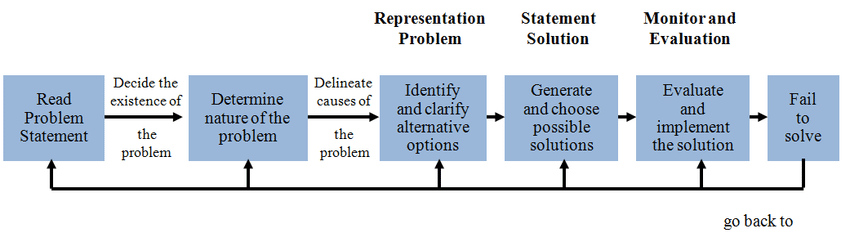
\includegraphics[scale=0.7]{ISP}
\end{center}
\subsection{Solutions}
\begin{itemize}
	\item Generate your initial boundaries - these are mutable
	\item From the initial limits, decompose the problem into smaller problems
	\item Identify potential solution criteria for the sub-problems
	\item Feedback, consider and reframe
\end{itemize}
In SE a good problem solver need the following:
\begin{itemize}
	\item \textbf{Method}: refers to a formal procedure; a formal "recipe" for accomplishing a goal that is typically independent of the tools used
	\item \textbf{Tool}: An instrument or automated system for accomplishing something in a better way
	\item \textbf{Procedure}: A combination of tools and techniques to produce a product
	\item \textbf{Paradigm}: A philosophy or approach for building a product
\end{itemize}
\section{Stakeholders}
\begin{itemize}
	\item Customer: The company, organization, or person who pays for the software system
	\item Developer: The company, organization or person who is building the software system
	\item User: The person or people who will actually use the system
\end{itemize}
\section{Where does the blame lie?}
Four factors identified for a higher chance of success:
\begin{itemize}
	\item User involvement
	\item Executive management support
	\item Clear requirement statements
	\item Proper planning
\end{itemize}
Three main factors identified in challenged or failed projects
\begin{itemize}
	\item Incomplete requirements/changing requirements
	\item Lack of user involvement/input
	\item Lack of resources
\end{itemize}
\section{SE Code of Ethics}
Code of ethics is not a formal checklist or exhaustive
\begin{itemize}
	\item To help us develop an understanding of what is appropriate
	\item Ethical rules and codes can only be used effectively by persons with good judgement
	\item Good judgement is acquired experience, good habits and conscious attention to ethical issues
	\item Exemplary software engineers have been described as having the following characteristics:
	\begin{itemize}
		\item Strong sense of individual responsibility; acute awareness of the world around them; brutal honesty; resilience under pressure; heightened sense of fairness; attention to detail
	\end{itemize}
\end{itemize}







\end{document}